\chapter{Rezoluce v predikátové logice} 
\label{chapter:predicate-resolution}

V této kapitole si ukážeme, jak lze adaptovat rezoluční metodu, kterou jsme představili v Kapitole \ref{chapter:propositional-resolution}, na predikátovou logiku. Tato kapitola, poslední v části o predikátové logice, je poměrně rozsáhlá, proto uveďme přehled její struktury: 

\begin{itemize}
    \item Začneme neformálním úvodem (Sekce \ref{section:predicate-resolution-intro}).
\end{itemize}
V následujících třech sekcích představíme nástroje, které nám umožní vypořádat se se specifiky predikátové logiky: s kvantifikátory, proměnnými a termy.
\begin{itemize}
    \item V Sekci \ref{section:skolemization} si ukážeme si, jak pomocí \emph{Skolemizace} odstranit kvantifikátory, abychom získali otevřené formule, které už lze převést do CNF.
    \item V Sekci \ref{section:grounding} vysvětlíme, že rezoluční zamítnutí bychom mohli hledat `na úrovni výrokové logiky' (tzv. \emph{grounding}), pokud bychom nejprve za proměnné substituovali `vhodné' konstantní termy.
    \item V Sekci \ref{section:unification} ukážeme, jak takové `vhodné' substituce hledat pomocí \emph{unifikačního algoritmu}.
\end{itemize}
Tím budeme mít všechny potřebné nástroje k představení vlastní rezoluční metody. Zbytek kapitoly má podobnou strukturu jako Kapitola \ref{chapter:propositional-resolution}.
\begin{itemize}
    \item Rezoluční pravidlo, rezoluční důkaz a související pojmy jsou popsány v Sekci \ref{section:predicate-resolution-method}.
    \item Sekce \ref{section:predicate-resolution-soundness-completeness} je věnována důkazu korektnosti a úplnosti.
    \item Na závěr, v Sekci \ref{section:predicate-LI-resolution}, popíšeme LI-rezoluci a její aplikaci v Prologu.
\end{itemize}


\section{Úvod}\label{section:predicate-resolution-intro}

Stejně jako ve výrokové logice, i v predikátové logice je rezoluční metoda založena na důkazu sporem. Chceme-li dokázat, že v teorii $T$ platí sentence $\varphi$ (tj. $T\models\varphi$), začneme s teorií $T\cup\{\neg \varphi\}$. Tuto teorii `převedeme' do CNF, a výslednou množinu klauzulí $S$ \emph{zamítneme} rezolucí (tj. ukážeme, že $S\proves_R\square$) čímž ukážeme, že je nesplnitelná.

Co myslíme konjunktivní normální formou? Roli \emph{literálu} hraje \emph{atomická formule}\footnote{Tj. $R(t_1,\dots,t_n)$ resp. $t_1=t_2$, kde $t_i$ jsou $L$-termy a $R$ je $n$-ární relační symbol z $L$.} nebo její negace. \emph{Klauzule} je (v množinové reprezentaci) konečná množina literálů, a \emph{formule} je množina klauzulí.\footnote{Jako ve výrokové logice připouštíme i nekonečné množiny klauzulí.} Jinak používáme stejnou terminologii, např. mluvíme o \emph{pozitivních}, \emph{negativních}, \emph{opačných} literálech, $\square$ značí prázdnou klauzuli (která je nesplnitelná), apod.

Nejprve si neformálně ukážeme specifika rezoluce v predikátové logice na několika velmi jednoduchých příkladech.

Všimněme si nejprve, že jsou-li teorie $T$ a sentence $\varphi$ \emph{otevřené} (neobsahují-li kvantifikátory), můžeme snadno sestrojit CNF formuli $S$ \emph{ekvivalentní} teorii $T\cup\{\neg \varphi\}$ (tj. mající stejnou množinu modelů). Nevadí ani univerzální kvantifikátory na začátku formule, ty můžeme odstranit beze změny významu.\footnote{Libovolná formule je ekvivalentní svému \emph{generálnímu uzávěru}, a ekvivalence platí oběma směry.}

\begin{example}
    Nechť $T=\{(\forall x)P(x),(\forall x)(P(x)\limplies Q(x))\}$ a $\varphi=(\exists x)Q(x)$. Je snadno vidět, že platí
    $$
    T\sim \{P(x),P(x)\limplies Q(x)\}\sim\{P(x),\neg P(x)\lor Q(x)\}
    $$ 
    a také:
    $$\neg\varphi=\neg(\exists x)Q(x)\sim(\forall x)\neg Q(x)\sim\neg Q(x)$$ 
    Teorii $T\cup\{\neg \varphi\}$ tedy můžeme převést na \emph{ekvivalentní} CNF formuli
    $$
    S = \{\{P(x)\},\{\neg P(x),Q(x)\},\{\neg Q(x)\}\}
    $$
    kterou snadno zamítneme rezolucí ve dvou krocích. (Představte si místo $P(x)$ výrokovou proměnnou $p$ a místo $Q(x)$ výrokovou proměnnou $q$.)
\end{example}

Obecně se nám to ale nepodaří, problémy dělá zejména existenční kvantifikátor. Na rozdíl od výrokové logiky \emph{není} každá teorie ekvivalentní CNF formuli. Ukážeme si ale postup, kterým lze vždy najít \emph{ekvisplnitelnou} CNF formuli, tj. takovou, která je nesplnitelná, \emph{právě když} $T\cup\{\neg \varphi\}$ je nesplnitelná, což nám k důkazu sporem stačí. Této konstrukci se říká \emph{Skolemizace} a spočívá v nahrazení existenčně kvantifikovaných proměnných nově přidanými konstantními resp. funkčními symboly. 

Například, formuli $(\exists x)\psi(x)$ nahradíme formulí $\psi(x/c)$, kde $c$ je nový konstantní symbol, který reprezentuje \emph{svědka}, tj. prvek, díky kterému je existenční kvantifikátor splněn. Protože takových prvků může být mnoho, ztrácíme \emph{ekvivalenci} teorií, platí ale, že je-li splnitelná původní formule, je splnitelná, i nová formule, a naopak.

\begin{example}
  Máme-li $T=\{(\exists x)P(x),P(x)\liff Q(x)\}$ a $\varphi=(\exists x)Q(x)$, potom 
  $$
  \neg\varphi\sim(\forall x)\neg Q(x)\sim\neg Q(x)
  $$
  a ekvivalenci můžeme převést do CNF jako obvykle, dostáváme:
  $$
  T\cup\{\neg \varphi\}\sim\{(\exists x)P(x),\neg P(x)\lor Q(x),\neg Q(x)\lor P(x),\neg Q(x)\}
  $$
  Formuli $(\exists x)P(x)$ nyní nahradíme $P(c)$, kde $c$ je nový konstantní symbol. Tím dostáváme CNF formuli:
  $$
  S = \{\{P(c)\},\{\neg P(x),Q(x)\},\{\neg Q(x),P(x)\},\{\neg Q(x)\}\}
  $$
  Ta není ekvivalentní teorii $T\cup\{\neg \varphi\}$, ale je s ní \emph{ekvisplnitelná} (v tomto případě jsou obě nesplnitelné).
\end{example}

Skolemizace může být i složitější, ne vždy stačí konstantní symbol. Pokud máme formuli tvaru $(\forall x)(\exists y)\psi(x,y)$, závisí zvolený svědek pro $y$ na zvolené hodnotě pro $x$, tedy `$y$ je funkcí $x$'. V tomto případě musíme $y$ nahradit $f(x)$, kde $f$ je nový unární funkční symbol. Tím dostáváme formuli $(\forall x)\psi(x,y/f(x))$ a univerzální kvantifikátor nyní můžeme odstranit a psát jen $\psi(x,y/f(x))$, což už je otevřená formule, byť v jiném jazyce (rozšířeném o symbol $f$). Skolemizaci formálně popíšeme, a potřebné vlastnosti dokážeme, v Sekci \ref{section:skolemization}. 

Nyní se podívejme na \emph{rezoluční pravidlo}. To je v predikátové logice složitější. Ukážeme si opět jen několik příkladů, formální definici necháme na později (Sekce \ref{section:predicate-resolution-method}).

\begin{example}
    V předchozím příkladu jsme dospěli k následující CNF formuli $S$, která je nesplnitelná, a chtěli bychom ji tedy rezolucí zamítnout:    
    $$
    S = \{\{P(c)\},\{\neg P(x),Q(x)\},\{\neg Q(x),P(x)\},\{\neg Q(x)\}\}
    $$
    Pokud bychom se na ni podívali `na úrovni výrokové logiky' (`ground level') a nahradili každou atomickou formuli novou výrokovou proměnnou, dostali bychom $\{\{r\},\{\neg p,q\},\{\neg q,p\},\{\neg q\}\}$, což není nesplnitelné. Potřebujeme využít toho, že $P(c)$ a $P(x)$ mají `podobnou strukturu' (jsou \emph{unifikovatelné}).

    Protože platí klauzule $\{\neg P(x),Q(x)\}$, platí i po provedení \emph{libovolné substituce}, tj. klauzule $\{\neg P(x/t),Q(x/t)\}$ je důsledkem $S$ pro libovolný term $t$. Mohli bychom si představit, že do  $S$ `přidáváme' všechny takto získané klauzule.\footnote{Těch je nekonečně mnoho, nekonečně mnoho je už jen \emph{variant} jedné klauzule, tj. klauzulí vzniklých pouhým přejmenováním proměnných. To nám ale nevadí, CNF formule může být dle definice nekonečná.} Výsledná CNF formule by po převedení na `úroveň výrokové logiky' už byla nesplnitelná. 
    
    \emph{Unifikační algoritmus} nám ale rovnou řekne, že správná substituce je $x/c$, a toto zahrneme už do \emph{rezolučního pravidla}, tedy \emph{rezolventou} klauzulí $\{P(c)\}$ a $\{\neg P(x),Q(x)\}$ bude klauzule $\{Q(c)\}$.
\end{example}

Unifikace může být i složitější, a upozorněme ještě na jeden rozdíl oproti výrokové logice: dovolíme si udělat rezoluci přes více literálů najednou, a to v případě, že jsou všechny dohromady \emph{unifikovatelné}:

\begin{example}
    Z klauzulí $\{R(x,f(x)),R(g(y),z)\}$ a $\{\neg R(g(c),u),P(u)\}$ (kde $R$ je binární relační, $f$ a $g$ jsou unární funkční, a $c$ konstantní symbol) bude možné odvodit rezolventu $\{P(f(g(c))\}$ za použití \emph{substituce} (\emph{unifikace}) $\{x/g(c),y/c,z/f(g(c)),u/f(g(c))\}$, kde z první klauzule vybíráme \emph{oba} literály najednou.
\end{example}

\begin{remark}
    To, že proměnné mají `lokální význam' v jednotlivých klauzulích (tj. můžeme za ně substituovat v jedné klauzuli aniž by to ovlivnilo ostatní klauzule), plyne z následující jednoduché tautologie, která platí pro libovolné formule $\psi,\chi$ (i pokud je v obou proměnná $x$ volná):
    $$
    \models(\forall x)(\psi \land \chi) \leftrightarrow (\forall x)\psi \land (\forall x)\chi
    $$
    
    Jak je vidět v předchozím příkladě, budeme také vyžadovat, aby klauzule v rezolučním pravidle měly disjunktní množiny proměnných; toho lze dosáhnout přejmenováním proměnných, což je speciální případ substituce.  
\end{remark}


\section{Skolemizace}\label{section:skolemization}

V této sekci ukážeme postup, jak redukovat otázku splnitelnosti dané teorie $T$ na otázku splnitelnosti \emph{otevřené} teorie $T'$. Připomeňme, že $T$ a $T'$ obecně nebudou ekvivalentní, budou ale \emph{ekvisplnitelné}:

\begin{definition}[Ekvisplnitelnost]
Mějme teorii $T$ v jazyce $L$ a teorii $T'$ v ne nutně stejném jazyce $L'$. Říkáme, že $T$ a $T'$ jsou \emph{ekvisplnitelné}, 
pokud platí: 
$$
\text{$T$ má model}\ \Leftrightarrow\ \text{$T'$ má model}
$$
\end{definition}

Celá konstrukce sestává z následujících kroků, které vysvětlíme níže:
\begin{enumerate}
    \item Převod do \emph{prenexní normální formy} (vytýkání kvantifikátorů).
    \item Nahrazení formulí jejich generálními uzávěry (abychom získali sentence).
    \item Odstranění existenčních kvantifikátorů (nahrazení sentencí \emph{Skolemovými variantami}).
    \item Odstranění zbývajících univerzálních kvantifikátorů (výsledkem jsou otevřené formule).
\end{enumerate}

\subsection{Prenexní normální forma}

Nejprve ukážeme postup, jakým můžeme z libovolné formule `vytknout' kvantifikátory, tj. převést do tzv. \emph{prenexní normální formy}, která začíná posloupností kvantifikátorů, a pokračuje už jen volnou formulí.

\begin{definition}[PNF]
    Formule $\varphi$ je v \emph{prenexní normální formě (PNF)}, je-li tvaru
    $$
    (Q_1x_1)\dots(Q_nx_n)\varphi'
    $$
    kde $Q_i$ je kvantifikátor ($\forall$ nebo $\exists$) a formule $\varphi'$ je otevřená. Formuli $\varphi'$ potom říkáme \emph{otevřené jádro} $\varphi$ a $(Q_1x_1)\dots(Q_nx_n)$ je \emph{kvantifikátorový prefix}. 
    
    Je-li $\varphi$ formule v PNF a jsou-li všechny kvantifikátory univerzální, potom říkáme, že $\varphi$ je \emph{univerzální} formule.
\end{definition}

Cílem této podsekce je ukázat následující tvrzení:

\begin{proposition}[Převod do PNF]\label{proposition:convert-to-pnf}
    Ke každé formuli $\varphi$ existuje ekvivalentní formule v prenexní normální formě.    
\end{proposition}

Algoritmus bude podobně jako převod do CNF založen na nahrazování podformulí \emph{ekvivalentními} podformulemi, s cílem posunout kvantifikátory blíže ke kořeni stromu formule. Co myslíme ekvivalencí formulí $\varphi\sim\varphi'$? To, že mají stejný význam, tj. v každém modelu a při každém ohodnocení proměnných mají touž pravdivostní hodnotu. Ekvivalentně, že platí $\models\varphi\liff\varphi'$. Budeme potřebovat následující jednoduché pozorování:

\begin{observation}\label{observation:pnf-one-step}
    Nahradíme-li ve formuli $\varphi$ nějakou podformuli $\psi$ ekvivalentní formulí $\psi'$, potom je i výsledná formule $\varphi'$ ekvivalentní formuli $\varphi$.
\end{observation}

Převod je založen na opakovaném použití následujících syntaktických pravidel:

\begin{lemma}\label{lemma:pnf-conversion-rules}
    Označme jako $\overline{Q}$ kvantifikátor opačný ke $Q$. Nechť $\varphi$ a $\psi$ jsou formule, a proměnná $x$ nechť není volná ve formuli $\psi$. Potom platí:
    \begin{align*}
        \neg (Qx)\varphi\ &\sim\ (\overline{Q}x)\neg\varphi\\
        (Qx)\varphi \land \psi\ &\sim\ (Qx)(\varphi \land \psi)\\
        (Qx)\varphi \lor \psi\ &\sim\ (Qx)(\varphi \lor \psi)\\
        (Qx)\varphi \limplies \psi\ &\sim\ (\overline{Q}x)(\varphi \limplies \psi)\\
        \psi \limplies (Qx)\varphi\ &\sim\ (Qx)(\psi \limplies \varphi)
    \end{align*}
\end{lemma}
\begin{proof}
    Pravidla lze snadno ověřit sémanticky, nebo dokázat tablo metodou (v tom případě nejde-li o sentence, musíme je nahradit jejich generálními uzávěry).   
\end{proof}

Všimněte si, že v pravidle $(Qx)\varphi \limplies \psi\sim(\overline{Q}x)(\varphi \limplies \psi)$ pro vytýkání z \emph{antecendentu} implikace musíme změnit kvantifikátor (z $\forall$ na $\exists$ a naopak) zatímco při vytýkání z \emph{konsekventu} zůstává kvantifikátor stejný. Proč tomu tak je vidíme nejlépe pokud přepíšeme implikaci pomocí disjunkce a negace:
$$
(Qx)\varphi \limplies \psi\sim\neg(Qx)\varphi \lor\psi\sim(\overline{Q}x)(\neg\varphi)\lor\psi\sim(\overline{Q}x)(\neg\varphi\lor\psi)\sim (\overline{Q}x)(\varphi \limplies \psi)
$$
Všimněte si také předpokladu, že $x$ není volná v $\psi$. Bez něj by pravidla nefungovala, viz např:
$$
(\exists x)P(x)\land Q(x)\ \not\sim\ (\exists x)(P(x)\land Q(x))
$$
V takové situaci nahradíme formuli variantou, ve které přejmenujeme vázanou proměnnou $x$ na nějakou novou proměnnou: 
$$
(\exists x)P(x)\land Q(x)\ \sim\ (\exists y)P(y)\land Q(x) \sim (\exists y)(P(y)\land Q(x))
$$
\begin{exercise}
    Dokažte Pozorování \ref{observation:pnf-one-step} a všechna pravidla z Lemmatu \ref{lemma:pnf-conversion-rules}.
\end{exercise}

Ukažme si postup na jednom příkladě:

\begin{example}\label{example:convert-to-pnf}
    Převeďme formuli $((\forall z)P(x,z)\land P(y,z))\ \limplies\ \neg(\exists x)P(x,y)$ do PNF. Zapíšeme jen jednotlivé mezikroky. Všimněte si, jaké pravidlo na jakou podformuli bylo použito (a také přejmenování proměnné v prvním kroku), a sledujte postup na stromu formule.
    \begin{align*}
        &\ (\forall z)P(x,z)\land P(y,z)\ \limplies\ \neg(\exists x)P(x,y)\\ \sim &\ 
        (\forall u) P(x,u)\land P(y,z)\ \limplies\ (\forall x)\neg P(x,y)\\ \sim &\ 
        (\forall u)(P(x,u)\land P(y,z))\ \limplies\ (\forall v)\neg P(v,y)\\ \sim &\ 
        (\exists u)( P(x,u)\land P(y,z)\ \limplies\ (\forall v)\neg P(v,y))\\ \sim &\ 
        (\exists u)(\forall v)( P(x,u)\land P(y,z)\ \limplies\ \neg P(v,y))
        \end{align*}    
\end{example}

Nyní nám již nic nebrání dokázat Tvrzení \ref{proposition:convert-to-pnf}:

\begin{proof}[Důkaz Tvrzení \ref{proposition:convert-to-pnf}]
    Indukcí podle struktury formule $\varphi$ s využitím Lemmatu \ref{lemma:pnf-conversion-rules} a Pozorování \ref{observation:pnf-one-step}.
\end{proof}

Protože je každá formule $\varphi(x_1,\dots,x_n)$ ekvivalentní svému \emph{generálnímu uzávěru} $$(\forall x_1)\dots(\forall x_n)\varphi(x_1,\dots,x_n)$$ můžeme Tvrzení \ref{proposition:convert-to-pnf} vyslovit také takto:

\begin{corollary}
    Ke každé formuli $\varphi$ existuje ekvivalentní \emph{sentence} v PNF.
\end{corollary} 

Například v Příkladu \ref{example:convert-to-pnf} je výsledná sentence $(\forall x)(\forall y)(\forall z)(\exists u)(\forall v)( P(x,u)\land P(y,z)\limplies\neg P(v,y))$.

\begin{remark}
    Prenexní forma není jednoznačná, pravidla pro převod můžeme aplikovat v různém pořadí. Jak uvidíme v následující podsekci, je výhodné vytýkat přednostně kvantifikátory [ze kterých se stanou] existenční: Máme-li na výběr mezi $(\forall x)(\exists y)\varphi(x,y)$ a $(\exists y)(\forall x)\varphi(x,y)$, volíme druhou variantu, neboť v první je `$y$ závislé na $x$'.
\end{remark}



\subsection{Skolemova varianta}

Nyní jsme převedli naše axiomy na ekvivalentní sentence v prenexním tvaru. Pokud by některá sentence obsahovala pouze univerzální kvantifikátory, tj. byla tvaru 
$$(\forall x_1)\dots(\forall x_n)\varphi(x_1,\dots,x_n)$$ 
kde $\varphi$ je otevřená, mohli bychom ji prostě nahradit jejím otevřeným jádrem $\varphi$, které je jí v tomto případě ekvivalentní. Jak si ale poradit s existenčními kvantifikátory, např. $(\exists x)\varphi(x)$, $(\forall x)(\exists y)\varphi(x,y)$, apod? Ty nejprve nahradíme jejich \emph{Skolemovou variantou}.

\begin{definition}[Skolemova varianta]
Mějme $L$-sentenci $\varphi$ v PNF, a nechť všechny její vázané proměnné jsou různé. Nechť existenční kvantifikátory z prefixu $\varphi$ jsou $(\exists y_1),\dots,(\exists y_n)$ (v tomto pořadí), a nechť pro každé $i$ jsou $(\forall x_1),\dots,(\forall x_{n_i})$ právě všechny univerzální kvantifikátory předcházející kvantifikátor $(\exists y_i)$ v prefixu $\varphi$. 

Označme $L'$ rozšíření $L$ o \emph{nové} $n_i$-ární funkční symboly $f_1,\dots,f_n$, kde symbol $f_i$ je arity $n_i$, pro každé $i$. \emph{Skolemova varianta} sentence $\varphi$ je $L'$-sentence $\varphi_S$ vzniklá z $\varphi$ tak, že pro každé $i=1,\dots,n$:
\begin{itemize}
    \item odstraníme z prefixu kvantifikátor $(\exists y_i)$, a
    \item substituujeme za proměnnou $y_i$ term $f_i(x_1,\dots,x_{n_i})$.
\end{itemize}
Tomuto procesu říkáme také \emph{skolemizace}.
\end{definition}

\begin{example}
    Skolemova varianta sentence 
    $$\varphi=(\exists y_1)(\forall x_1)(\forall x_2)(\exists y_2)(\forall x_3)R(y_1,x_1,x_2,y_2,x_3)$$
    je sentence
    $$
    \varphi_S=(\forall x_1)(\forall x_2)(\forall x_3)R(f_1,x_1,x_2,f_2(x_1,x_2),x_3)
    $$
    kde $f_1$ je nový konstantní symbol a $f_2$ je nový binární funkční symbol.
\end{example}

\begin{remark}
    Nezapomeňte, že při skolemizaci musíme vycházet ze sentence! Napříkla máme-li formuli $(\exists y)E(x,y)$, není $E(x,c)$ její Skolemova varianta. Musíme napřed provést generální uzávěr $(\forall x)(\exists y)E(x,y)$, a potom správně skolemizovat jako $(\forall x)E(x,f(x))$, což je ekvivalentní otevřené formuli $E(x,f(x))$ (která říká něco mnohem slabšího než $E(x,c)$).

    Je také důležité, aby každý symbol použitý při skolemizaci byl opravdu nový, jeho jedinou `rolí' v celé teorii musí být reprezentovat `existující' prvky v této formuli.
\end{remark} 

V následujícím lemmatu ukážeme klíčovou vlastnost skolemovy varianty:

\begin{lemma}\label{lemma:skolem-variant-conservative-extension}
Mějme $L$-sentenci $\varphi=(\forall x_1)\dots(\forall x_n)(\exists y)\psi$ a nechť $\varphi'$ je sentence $\varphi=(\forall x_1)\dots(\forall x_n)\psi(y/f(x_1,\dots,x_n))$, kde $f$ je nový funkční symbol. Potom:
\begin{enumerate}[(i)]
    \item $L$-redukt každého modelu $\varphi'$ je modelem $\varphi$, a 
    \item každý model $\varphi$ lze expandovat na model $\varphi'$.
\end{enumerate}
\end{lemma}

\begin{proof}
    Nejprve dokažme část (i): Mějme model $\A'\models\varphi'$ a nechť $\A$ je jeho redukt na jazyk $L$. Pro každé ohodnocení proměnných $e$ platí $\A\models\psi[e(y/a)]$ pro $a=(f(x_1,\dots,x_n))^{\A'}[e]$, tedy $\A\models\varphi$.
    
    Nyní část (ii): Protože $\A\models\varphi$, existuje funkce $f^A:A^n\to A$ taková, že pro každé ohodnocení proměnných $e$ platí $\A\models \psi[e(y/a)]$, kde $a=f^A(e(x_1),\dots,e(x_n))$. To znamená, že expanze struktury $\A$ vzniklá přidáním funkce $f^A$ je modelem $\varphi'$.    
\end{proof}

\begin{remark}
    Expanze modelu ve druhé části tvrzení nemusí být (a typicky není) jednoznačná, na rozdíl od extenze o definici nového funkčního symbolu.
\end{remark}

Aplikujeme-li předchozí lemma opakovaně (postupně pro všechny existenční kvantifikátory), získáme následující důsledek:

\begin{corollary}
    Sentence $\varphi$ a její skolemova varianta $\varphi_S$ jsou ekvisplnitelné.
\end{corollary}


\subsection{Skolemova věta}

V této podsekci shrneme celý postup popsaný v předchozích podsekcích. Klíčem je následující věta norského logika Thoralfa Skolema:

\begin{theorem}[Skolemova věta]
    Každá teorie má otevřenou konzervativní extenzi.
\end{theorem}
\begin{proof}
    Mějme $L$-teorii $T$. Každý axiom nahradíme jeho generálním uzávěrem (není-li to už sentence) a převedeme do PNF, tím získáme ekvivalentní teorii $T'$. Nyní nahradíme každý axiom teorie $T'$ jeho Skolemovou variantou. Tím získáme teorii $T''$ v rozšířeném jazyce $L'$. Z Lemmatu \ref{lemma:skolem-variant-conservative-extension} plyne, že $L$-redukt každého modelu $T''$ je modelem $T'$, tedy $T''$ je extenzí $T'$, a že každý model $T'$ lze expandovat do jazyka $L'$ na model $T''$, tedy jde o konzervativní extenzi. Teorie $T''$ je axiomatizovaná univerzálními sentencemi, odstraníme-li kvantifikátorové prefixy (tj. vezmeme-li jádra axiomů), získáme ekvivalentní otevřenou teorii $T'''$, která je hledanou konzervativní extenzí.
\end{proof}

Ze sémantické charakterizace konzervativní extenze snadno plyne následující důsledek:

\begin{corollary}
    Ke každé teorii existuje ekvisplnitelná otevřená teorie.
\end{corollary}

Otevřenou teorii už můžeme snadno převést do CNF (vyjádřit \emph{formulí} $S$ v množinové reprezentaci) pomocí ekvivalentních syntaktických úprav, stejně jako ve výrokové logice (viz Sekce \ref{subsection:convert-to-normal-form}).


\section{Grounding}\label{section:grounding}

V této sekci si ukážeme, že máme-li otevřenou teorii, která je nesplnitelná, můžeme její nesplnitelnost doložit `na konkrétních prvcích'. Co tím myslíme? Existuje konečně mnoho \emph{základních (ground) instancí} axiomů (instancí, kde za proměnné substituujeme konstantní termy), takových, že jejich konjunkce (která neobsahuje žádnou proměnnou) je nesplnitelná. 

\begin{definition}[Základní instance]
    Mějme otevřenou formuli $\varphi$ ve volných proměnných $x_1,\dots,x_n$. Řekneme, že instance $\varphi(x_1/t_1,\dots,x_n/t_n)$ je \emph{základní (ground) instance}, jsou-li všechny termy $t_1,\dots,t_n$ konstantní (ground).
\end{definition}

\begin{example}
    Teorie $T=\{P(x,y)\lor R(x,y),\neg P(c,y),\neg R(x,f(x))\}$ v jazyce $L=\langle P,R,f,c \rangle$ nemá model. Můžeme to doložit následující konjunkcí základních instancí axiomů, kde za proměnnou $x$ substituujeme konstantu $c$ a za $y$ konstantní term $f(c)$:
$$
(P(c,f(c))\lor R(c,f(c)))\ \land\ \neg P(c,f(c))\ \land\ \neg R(c,f(c))
$$
\end{example}
Tato sentence je zjevně nesplnitelná. Základní atomické sentence $(P(c,f(c))$ a $R(c,f(c))$ můžeme navíc (díky tomu, že neobsahují proměnné) chápat jako výrokové proměnné $p_1,p_2$, kde $p_1$ znamená `platí $P(c,f(c))$' a $p_2$ znamená `platí $R(c,f(c))$'. Dostáváme potom následující výrok, který lze snadno zamítnout rezolucí:
$$
(p_1 \lor p_2) \land \neg p_1 \land \neg p_2
$$
Tomuto procesu převedení na základní instance (a tím do výrokové logiky) říkáme `grounding'. Za chvíli ho zformalizujeme a dokážeme \emph{Herbrandovu větu},\footnote{Francouzský matematik Jacques Herbrand pracoval na konci 20. let 20. století. Během své krátké kariéry (zemřel tragicky ve věku 23 let) objevil několik dalších důležitých výsledků, a mimo jiné formalizoval pojem rekurzivní funkce.} která říká, že taková nesplnitelná konjunkce základních instancí axiomů existuje pro každou nesplnitelnou teorii.

\subsection{Přímá redukce do výrokové logiky}

Uvědomme si nyní, že díky Herbrandově větě grounding umožňuje následující postup, byť neefektivní, jak zamítat formule rezolucí `na úrovni výrokové logiky': Ve vstupní formuli $S$ nahradíme každou klauzuli množinou všech jejích základních instancí (pokud žádné nejsou, tedy pokud jazyk neobsahuje konstantní symbol, jeden konstantní symbol do jazyka přidáme). Ve výsledné množině klauzulí $S'$ chápeme atomické sentence jako výrokové proměnné, a $S'$ zamítneme výrokovou rezolucí (o které víme, že je korektní a úplná). 

Problémem tohoto přístupu je, že klauzulí v $S'$ (základních instancí klauzulí s $S$ může být mnoho, i nekonečně mnoho, např. kdykoliv je v jazyce alespoň jeden funkční (nekonstantní) symbol. 

\begin{example}
Máme-li CNF formuli $S=\{\{P(x,y),R(x,y)\},\{\neg P(c,y)\},\{\neg R(x,f(x))\}\}$ v jazyce $L=\langle f,c\rangle$, nahradíme ji následující nekonečnou formulí $S'$:
\begin{align*}
    S'=\{&\{P(c,c),R(c,c)\},\{P(c,f(c)),R(c,f(c))\},\{P(f(c),c),R(f(c),c)\},\dots,\\ 
    &\{\neg P(c,c)\}, \{\neg P(c,f(c))\},\{\neg P(c,f(f(c)))\},\{\neg P(c,f(f(f(c))))\}, \dots,\\
    &\{\neg R(c,f(c))\}, \{\neg R(f(c),f(f(c)))\},\{\neg R(f(f(c)),f(f(f(c))))\},\dots\}    
\end{align*}
Ta je nesplnitelná, neboť obsahuje následující konečnou podmnožinu, která je nesplnitelná, což snadno ukážeme výrokovou rezolucí:
$$
\{\{P(c,f(c)),R(c,f(c))\},\{\neg P(c,f(c))\},\{\neg R(c,f(c))\}\}\proves_R\square
$$
\end{example}
V Sekci \ref{section:unification} si ukážeme efektivní postup jak hledat vhodné základní instance klauzulí, pomocí tzv. \emph{unifikace}.


\subsection{Herbrandova věta}

V této podsekci vyslovíme a dokážeme Herbrandovu větu. Budeme předpokládat, že jazyk obsahuje nějaký konstantní symbol: pokud v jazyce žádný není, jeden přidáme. Konstantní symbol potřebujeme k tomu, aby existovaly konstantní termy, a my mohli vytvořit tzv. \emph{Herbrandův model}. Jde o konstrukci sémantického objektu (modelu) ze syntaktických objektů (konstantních termů) velmi podobnou \emph{kanonickému modelu} (Definice \ref{definition:canonical-model-predicate}).\footnote{Rozdíl je v tom, že nepřidáváme spočetně mnoho nových konstantních symbolů (vycházíme jen z konstantních symbolů, které už v jazyce jsou), a také nijak nepředepisujeme, jak mají vypadat relace modelu.}

\begin{definition}[Herbrandův model]
Mějme jazyk $L=\langle\mathcal R,\mathcal F\rangle$ s alespoň jedním konstantním symbolem. $L$-struktura $\A=\langle A,\mathcal R^\A,\mathcal F^\A\rangle$ je \emph{Herbrandův model}, jestliže:
\begin{itemize}
    \item $A$ je množina všech konstantních $L$-termů (tzv. \emph{Herbrandovo univerzum}), a
    \item pro každý $n$-ární funkční symbol $f\in\mathcal F$ a konstantní termy $\text{``$t_1$''},\dots,\text{``$t_n$''}\in A$ platí:
    $$
    f^\A(\text{``$t_1$''},\dots,\text{``$t_n$''})=\text{``$f(t_1,\dots,t_n)$''}
    $$
    \item Speciálně, pro každý konstantní symbol $c\in\mathcal F$ je $c^\A=\text{``$c$''}$.
\end{itemize}
Na interpretace relačních symbolů neklademe žádné podmínky.
\end{definition}

Připomeňme, že uvozovky okolo termů píšeme jen neformálně, abychom jasněji odlišili termy jako syntaktické objekty (řetězce symbolů) od jejich interpretací (funkcí).

\begin{example}
Mějme jazyk $L=\langle P,f,c\rangle$, kde $P$ je unární relační, $f$ je binární funkční, a $c$ konstantní symbol. Herbrandovo univerzum pro tento jazyk je množina
$$
A=\{\text{``$c$''},\text{``$f(c,c)$''},\text{``$f(c,f(c,c))$''},\text{``$f(f(c,c),c)$''}\dots\}
$$
Struktura $\A=\langle A,P^\A,f^\A,c^\A\rangle$ je Herbrandův model, jestliže $c^\A=\text{``$c$''}$ a funkce $f^\A$ splňuje:
\begin{itemize}
    \item $f^\A(\text{``$c$''},\text{``$c$''})=\text{``$f(c,c)$''}$,
    \item $f^\A(\text{``$c$''},\text{``$f(c,c)$''})=\text{``$f(c,f(c,c))$''}$,
    \item $f^\A(\text{``$f(c,c)$''},\text{``$c$''})=\text{``$f(f(c,c),c)$''}$, atd.
\end{itemize}
Relace $P^\A$ může být libovolná podmnožina $A$.
\end{example}

Nyní jsme připraveni vyslovit Herbrandovu větu. Neformálně řečeno, je-li teorie splnitelná, tj. má-li model, potom má dokonce Herbrandův model, a v opačném případě najdeme nesplnitelnou konjunkci základních instancí axiomů, použitelnou pro rezoluční zamítnutí `na úrovni výrokové logiky'.


\begin{theorem}[Herbrandova věta]
Mějme otevřenou teorii $T$ v jazyce $L$ bez rovnosti a s alespoň jedním konstantním symbolem. Potom buď má $T$ \emph{Herbrandův model}, nebo existuje konečně mnoho základních instancí axiomů $T$, jejichž konjunkce je nesplnitelná.
\end{theorem}
\begin{proof}
Označme jako $T_\text{ground}$ množinu všech základních instancí axiomů teorie $T$. Zkonstruujeme systematické\footnote{Nebo libovolné dokončené tablo, ale tak, abychom sporné větve už neprodlužovali.} tablo z teorie $T_\text{ground}$ s položkou $\F\bot$ v kořeni, ale z jazyka $L$, bez rozšíření o pomocné konstantní symboly na jazyk $L_C$. 

Pokud tablo obsahuje bezespornou větev, potom je kanonický model pro tuto větev (opět bez přidání pomocných konstantních symbolů) Herbrandovým modelem $T$. V opačném případě máme tablo důkaz sporu, tedy teorie $T_\text{ground}$, a tím pádem i $T$, je nesplnitelná. Protože je tablo důkaz konečný, použili jsme v něm jen konečně mnoho základních instancí axiomů $\alpha_\text{ground}\in T_\text{ground}$. Jejich konjunkce je tedy nesplnitelná.
\end{proof}

\begin{remark}
Máme-li jazyk s rovností, potom nejprve teorii $T$ rozšíříme o axiomy rovnosti na teorii $T^*$, a má-li $T^*$ Herbrandův model $\A$, faktorizujeme ho podle kongruence $=^A$, stejně jako v případě kanonického modelu.
\end{remark}

Na závěr této sekce vyslovíme dva důsledky Herbrandovy věty.

\begin{corollary}
    Mějme otevřenou formuli $\varphi(x_1,\dots,x_n)$ v jazyce $L$ s alespoň jedním konstantním symbolem. Potom existují konstantní $L$-termy $t_{ij}$ ($1\leq i\leq m,1\leq j\leq n$) takové, že sentence 
    $$
    (\exists x_1)\dots(\exists x_n)\varphi(x_1,\dots,x_n)$$ 
    je pravdivá, právě když je následující formule (výroková) tautologie:
    $$
    \varphi(x_1/t_{11},\dots,x_n/t_{1n})\lor \dots \lor \varphi(x_1/t_{m1},\dots,x_n/t_{mn})
    $$
\end{corollary}
\begin{proof}
Sentence $(\exists x_1)\dots(\exists x_n)\varphi(x_1,\dots,x_n)$ je pravdivá, právě když $(\forall x_1)\dots(\forall x_n)\neg\varphi$ je nesplnitelná, neboli když $\neg\varphi$ je nesplnitelná. Tvrzení plyne z Herbrandovy věty aplikované na formuli $\neg\varphi$.
\end{proof}

\begin{corollary}
    Mějme otevřenou teorii $T$ v jazyce s alespoň jedním konstantním symbolem. Teorie $T$ má model, právě když má model teorie $T_\text{ground}$ sestávající ze všech základních instancí axiomů teorie $T$.
\end{corollary}
\begin{proof}
V modelu teorie $T$ platí všechny axiomy, tedy i všechny základní instance axiomů. Je tedy i modelem $T_\text{ground}$. Pokud $T$ nemá model, podle Herbrandovy věty je nějaká konečná podmnožina teorie $T_\text{ground}$ nesplnitelná.
\end{proof}


\section{Unifikace}\label{section:unification}
\todo

\subsection{Substituce}\todo

% from slides:
\subsubsection*{Substituce - příklady}
    
    {\it Efektivnější je využívat vhodných substitucí. Např. pro}
    \smallskip
    
    \begin{enumerate}
    \item[$a)$] \mygreen{$\{P(x),Q(x,a)\}$}, \mygreen{$\{\neg P(y),\neg Q(b,y)\}$} substitucí \mygreen{$x/b$}, \mygreen{$y/a$} dostaneme
    \smallskip
    
    \mygreen{$\{P(b),Q(b,a)\}$}, \mygreen{$\{\neg P(a),\neg Q(b,a)\}$} a z nich rezolucí \mygreen{$\{P(b),\neg P(a)\}$}.
    \medskip
    
    Nebo substitucí \mygreen{$x/y$} a rezolucí dle \mygreen{$P(y)$} dostaneme \mygreen{$\{Q(y,a),\neg Q(b,y)\}$}.
    \medskip
    
    \item[$b)$] \mygreen{$\{P(x),Q(x,a),Q(b,y)\}$}, \mygreen{$\{\neg P(v),\neg Q(u,v)\}$} substituce \mygreen{$x/b$}, \mygreen{$y/a$}, \mygreen{$u/b$}, \mygreen{$v/a$}
    \smallskip
    
    dává \mygreen{$\{P(b),Q(b,a)\}$}, \mygreen{$\{\neg P(a),\neg Q(b,a)\}$} a z nich rezolucí \mygreen{$\{P(b),\neg P(a)\}$}.
    \medskip
    
    \item[$c)$] \mygreen{$\{P(x),Q(x,z)\}$}, \mygreen{$\{\neg P(y),\neg Q(f(y),y)\}$} substitucí \mygreen{$x/f(z)$}, \mygreen{$y/z$} dostaneme
    \smallskip
    
    \mygreen{$\{P(f(z)),Q(f(z),z)\}$}, \mygreen{$\{\neg P(z),\neg Q(f(z),z)\}$} a z nich \mygreen{$\{P(f(z)),\neg P(z)\}$}.
    \medskip
    
    Při substituci \mygreen{$x/f(a)$}, \mygreen{$y/a$}, \mygreen{$z/a$} dostaneme \mygreen{$\{P(f(a)),Q(f(a),a)\}$},
    \smallskip
    
    \mygreen{$\{\neg P(a),\neg Q(f(a),a)\}$} a z nich rezolucí \mygreen{$\{P(f(a)),\neg P(a)\}$}. Předchozí
    \smallskip
    
    substituce je ale \myblue{obecnější}.
    \end{enumerate}
    
    
    
    %%%%%%%%%%%%%%%%%%%%%%%%%%%%%%%%%%%%%%%%%%%%%%%%%%%%%%5
    
    \subsubsection*{Substituce}
    
    \begin{itemize}
    \item \mdef{Substituce} je (konečná) množina \mygreen{$\sigma=\{x_1/t_1,\dots,x_n/t_n\}$}, kde $x_i$ jsou
    \smallskip
    
    \myblue{navzájem  různé} proměnné a $t_i$ jsou termy, přičemž $t_i$ \myblue{není} $x_i$.
    \smallskip
    
    \item Jsou-li všechny termy $t_i$ konstantní, je $\sigma$ \mdef{základní substituce}.
    \smallskip
    
    \item Jsou-li $t_i$ navzájem různé proměnné, je $\sigma$ \mdef{přejmenování proměnných}.
    \smallskip
    
    \item \mdef{Výraz} je literál nebo term. \emph{(Substituci lze aplikovat na výrazy.)}
    \smallskip
    
    \item \mdef{Instance} výrazu $E$ \mdef{při substituci} \mygreen{$\sigma=\{x_1/t_1,\dots,x_n/t_n\}$} je výraz \mdef{$E\sigma$}
    \smallskip
    
    vzniklý z $E$ \myblue{současným} nahrazením \myblue{všech} výskytů proměnných $x_i$ za $t_i$.
    \smallskip
    
    \item Pro množinu výrazů $S$ označme \mdef{$S\sigma$} množinu instancí $E\sigma$ výrazů $E$ z $S$.
    \end{itemize}
    \smallskip
    
    {\it \myblue{Poznámka}\ \ Jelikož substituce je současná pro všechny proměnné zároveň,
    \smallskip
    
    případný výskyt proměnné $x_i$ v termu $t_j$ nevede k zřetězení substitucí.}
    \medskip
    
    \mygreen{\it Např. pro $S=\{P(x),R(y,z)\}$ a substituci $\sigma=\{x/f(y,z),y/x,z/c\}$ je
    \vspace{-2mm}
    $$S\sigma=\{P(f(y,z)),R(x,c)\}.$$}
    
    \vspace{-6mm}
    
    
    %%%%%%%%%%%%%%%%%%%%%%%%%%%%%%%%%%%%%%%%%%%%%%%%%%%%%%5
    
    \subsubsection*{Skládání substitucí}
    {\it Zadefinujeme $\sigma\tau$ tak, aby $E(\sigma\tau)=(E\sigma)\tau$ pro každý výraz $E$.}
    \medskip
    
    \mygreen{\it Např. pro $E=P(x,w,u)$, $\sigma=\{x/f(y),w/v\}$, $\tau=\{x/a,y/g(x),v/w,u/c\}$ je}
    \vspace{-2mm}
    \mygreen{$$E\sigma=P(f(y),v,u),\quad(E\sigma)\tau=P(f(g(x)),w,c).$$}
    
    \vspace{-6mm}
    \mygreen{\it Pak by mělo být $\sigma\tau=\{x/f(g(x)),y/g(x),v/w,u/c\}$.}
    \bigskip
    
    Pro substituce \mygreen{$\sigma=\{x_1/t_1,\dots,x_n/t_n\}$} a \mygreen{$\tau=\{y_1/s_1,\dots,y_n/s_n\}$} definujeme
    \vspace{-1mm}
  $$\\sigma\tau=\{x_i/t_i\tau\mid x_i\in X,\text{ $x_i$ není $t_i\tau$}\}\cup\{y_j/s_j\mid y_j\in Y\setminus X\}$$
    
    \vspace{-5mm}
    \mdef{složenou substituci} $\sigma$ a $\tau$, kde $X=\{x_1,\dots,x_n\}$ a $Y=\{y_1,\dots,y_m\}$.
    \bigskip
    
    {\it \myblue{Poznámka}\ \ Skládání substitucí není komutativní, např. pro uvedené $\sigma$ a $\tau$ je}
    \vspace{-2mm}
    \mygreen{$$\tau\sigma=\{x/a,y/g(f(y)),u/c,w/v\}\ne \sigma\tau.$$}
    
    \vspace{-6mm}
    
    
    %%%%%%%%%%%%%%%%%%%%%%%%%%%%%%%%%%%%%%%%%%%%%%%%%%%%%%5
    
    \subsubsection*{Skládání substitucí - vlastnosti}
    {\it Ukážeme, že definice vyhovuje našemu požadavku a skládání je asociativní.}
    \medskip
    
    {\bf \myblue{Tvrzení}}\ \ {\it Pro každý výraz $E$ a substituce $\sigma$, $\tau$, $\varrho$ platí}
    \begin{enumerate}
    \item[$(i)$] \mygreen{$(E\sigma)\tau=E(\sigma\tau)$},
    \item[$(ii)$] \mygreen{$(\sigma\tau)\varrho=\sigma(\tau\varrho)$}.
    \end{enumerate}
    \medskip
    
    {\it \myblue{Důkaz}}\ \ Nechť \mygreen{$\sigma=\{x_1/t_1,\dots,x_n/t_n\}$} a \mygreen{$\tau=\{y_1/s_1,\dots,y_m/s_m\}$}. Stačí uvážit
    \smallskip
    
    případ, kdy $E$ je proměnná, řekněme $v$.
    \smallskip
    
    \begin{enumerate}
    \item[$(i)$] Je-li $v$ proměnná $x_i$ pro nějaké $i$, je \mygreen{$v\sigma=t_i$} a \mygreen{$(v\sigma)\tau=t_i\tau$}, což je $v(\sigma\tau)$
    \smallskip
    
    dle definice $\sigma\tau$. Jinak \mygreen{$v\sigma=v$} a \mygreen{$(v\sigma)\tau=v\tau$}.
    \smallskip
    
    \item[] Je-li $v$ proměnná $y_j$ pro nějaké $j$, je dále \mygreen{$(v\sigma)\tau=v\tau=s_j$}, což je $v(\sigma\tau)$
    \smallskip
    
    dle definice $\sigma\tau$. Jinak \mygreen{$(v\sigma)\tau=v\tau=v$} a zároveň \mygreen{$v(\sigma\tau)=v$}.
    \smallskip
    
    \item[$(ii)$] Opakovaným užitím $(i)$ dostaneme pro každý výraz $E$,
    \vspace{-2mm}
    \mygreen{$$E((\sigma\tau)\varrho)=(E(\sigma\tau))\varrho=((E\sigma)\tau)\varrho=(E\sigma)(\tau\varrho)=E(\sigma(\tau\varrho)).\quad\qed$$}
    
    \vspace{-6mm}
    \end{enumerate}
    
% :from slides

\subsection{Unifikační algoritmus}\todo

% from slides:
\subsubsection*{Unifikace}
    Nechť \mygreen{$S=\{E_1,\dots,E_n\}$} je (konečná) množina výrazů.
    \smallskip
    
    \begin{itemize}
    \item \mdef{Unifikace} pro $S$ je substituce $\sigma$ taková, že \mygreen{$E_1\sigma=E_2\sigma=\cdots =E_n\sigma$},
    \smallskip
    
    tj. $S\sigma$ je singleton.
    \smallskip
    
    \item $S$ je \mdef{unifikovatelná}, pokud má unifikaci.
    \smallskip
    
    \item Unifikace $\sigma$ pro $S$ je \mdef{nejobecnější unifikace (mgu)}, pokud pro každou
    \smallskip
    
    unifikaci $\tau$ pro $S$ existuje substituce $\lambda$ taková, že \mygreen{$\tau=\sigma\lambda$}.
    \end{itemize}
    \medskip
    
    \mygreen{\it Např. $S=\{P(f(x),y),P(f(a),w)\}$ je unifikovatelná pomocí nejobecnější}
    \smallskip
    
    \mygreen{unifikace $\sigma=\{x/a,y/w\}$. Unifikaci $\tau=\{x/a,y/b,w/b\}$ dostaneme jako $\sigma\lambda$}
    \smallskip
    
    \mygreen{pro $\lambda=\{w/b\}$. $\tau$ není mgu, nelze z ní získat unifikaci $\varrho=\{x/a, y/c, w/c\}$.}
    \bigskip
    
    {\it \myblue{Pozorování}\ \ Jsou-li $\sigma$, $\tau$ různé nejobecnější unifikace pro $S$, liší se pouze
    \smallskip
    
    \myblue{přejmenováním proměnných}.}
    
    
    %%%%%%%%%%%%%%%%%%%%%%%%%%%%%%%%%%%%%%%%%%%%%%%%%%%%%%5
    
    \subsubsection*{Unifikační algoritmus}
    Nechť $S$ je (konečná) neprázdná množina výrazů a $p$ je \myblue{nejlevější} pozice,
    \smallskip
    
    na které se nějaké dva výrazy z $S$ liší. Pak \mdef{neshoda} v $S$ je množina \mdef{$D(S)$}
    \smallskip
    
    podvýrazů začínajících na pozici $p$ ze \myblue{všech} výrazů v $S$ .
    \medskip
    
    \mygreen{\it Např. pro $S=\{P(x,y),P(f(x),z),P(z,f(x))\}$ je $D(S)=\{x,f(x),z\}.$}
    \bigskip
    
    {\it \myblue{Vstup}}\ \ Neprázdná (konečná) množina výrazů $S$.
    \smallskip
    
    {\it \myblue{Výstup}}\ \ Nejobecnější unifikace $\sigma$ pro $S$ nebo \emph{``$S$ není unifikovatelná''}.
    %\smallskip
    
    \begin{enumerate}
    \item[$(0)$] Nechť $S_0:=S$, $\sigma_0:=\emptyset$, $k:=0$. \hfill\emph{(inicializace)}
    \smallskip
    
    \item[$(1)$] Je-li $S_k$ singleton, vydej substituci $\sigma=\sigma_0\sigma_1\cdots \sigma_k$. \hfill\emph{(mgu pro $S$)}
    \smallskip
    
    \item[$(2)$] Zjisti, zda v $D(S_k)$ existuje proměnná $x$ a term $t$ \myblue{neobsahující} $x$.
    \smallskip
    
    \item[$(3)$] Pokud ne, vydej \emph{``$S$ není unifikovatelná''}.
    \smallskip
    
    \item[$(4)$] Jinak $\sigma_{k+1}:=\{x/t\}$, $S_{k+1}:=S_k\sigma_{k+1}$, $k:=k+1$ a jdi na $(1)$.
    \end{enumerate}
    \smallskip
    
    {\it \myblue{Poznámka}\ \ Test výskytu proměnné $x$ v termu $t$ v kroku $(2)$ může být \emph{``drahý''}.}% Např. implementace Prologu od něj upouštějí.}
    
    
    %%%%%%%%%%%%%%%%%%%%%%%%%%%%%%%%%%%%%%%%%%%%%%%%%%%%%%5
    
    \subsubsection*{Unifikační algoritmus - příklad}
     \vspace{-2mm}
    \mygreen{$$S=\{P(f(y,g(z)),h(b)),\ P(f(h(w),g(a)),t),\ P(f(h(b),g(z)),y)\}$$}
    
    \vspace{-5mm}
    \begin{enumerate}
    \item[$1)$] $S_0=S$ není singleton a $D(S_0)=\{y,h(w),h(b)\}$ obsahuje term $h(w)$ a
    \smallskip
    
    proměnnou $y$ nevyskytující se v $h(w)$. Pak $\sigma_1=\{y/h(w)\}$,  $S_1=S_0\sigma_1$, tj.
        \vspace{-2mm}
        \mygreen{$$S_1=\{P(f(h(w),g(z)),h(b)),\ P(f(h(w),g(a)),t),\ P(f(h(b),g(z)),h(w))\}.$$}
    
        \vspace{-6mm}
    \item[$2)$] $D(S_1)=\{w,b\}$, $\sigma_2=\{w/b\}$, $S_2=S_1\sigma_2$, tj.
    \vspace{-2mm}
        \mygreen{$$S_2=\{P(f(h(b),g(z)),h(b)),\ P(f(h(b),g(a)),t)\}.$$}
    
        \vspace{-6mm}
    \item[$3)$] $D(S_2)=\{z,a\}$, $\sigma_3=\{z/a\}$, $S_3=S_2\sigma_3$, tj.
    \vspace{-2mm}
        \mygreen{$$S_3=\{P(f(h(b),g(a)),h(b)),\ P(f(h(b),g(a)),t)\}.$$}
    
        \vspace{-6mm}
    \item[$4)$] $D(S_3)=\{h(b),t\}$, $\sigma_4=\{t/h(b)\}$, $S_4=S_3\sigma_4$, tj.
    \vspace{-2mm}
        \mygreen{$$S_4=\{P(f(h(b),g(a)),h(b))\}.$$}
    
        \vspace{-6mm}
    \item[$5)$] $S_4$ je singleton a nejobecnější unifikace pro $S$ je
    \vspace{-2mm}
        \mygreen{$$\sigma=\{y/h(w)\}\{w/b\}\{z/a\}\{t/h(b)\}=\{y/h(b),w/b,z/a,t/h(b)\}.$$}
    
        \vspace{-6mm}
    \end{enumerate}
    
    
    %%%%%%%%%%%%%%%%%%%%%%%%%%%%%%%%%%%%%%%%%%%%%%%%%%%%%%5
    
    \subsubsection*{Unifikační algoritmus - korektnost}
    {\bf \myblue{Tvrzení}}\ \ {\it Pro každé $S$ unifikační algoritmus vydá po konečně mnoha krocích
    \smallskip
    
    korektní výsledek, tj. nejobecnější unifikaci $\sigma$ pro $S$ nebo pozná, že $S$ není
    \smallskip
    
    unifikovatelná. $(*)$ Navíc, pro každou unifikaci $\tau$ pro $S$ platí, že \myblue{$\tau=\sigma\tau$}.}
    \medskip
    
    {\it \myblue{Důkaz}}\ \ V každém kroku eliminuje jednu proměnnou, někdy tedy skončí.
    %\vspace{0.5mm}
    
    \begin{itemize}
    \item Skončí-li neúspěchem po $k$ krocích, nelze unifikovat $D(S_k)$, tedy ani $S$.
    %\smallskip
    \vspace{0.5mm}
    
    \item Vydá-li $\sigma=\sigma_0\sigma_1\cdots\sigma_k$, je $\sigma$ evidentně \myblue{unifikace} pro $S$.
    %\smallskip
    \vspace{0.5mm}
    
    \item Dokážeme-li, že $\sigma$ má vlastnost $(*)$, je $\sigma$ \myblue{nejobecnější} unifikace pro $S$.
    %\smallskip
    \vspace{0.5mm}
    
    \item[$(1)$] Nechť $\tau$ je unifikace pro $S$. Ukážeme, že $\tau=\sigma_0\sigma_1\cdots\sigma_i\tau$ pro každé $i\le k$.
    %\smallskip
    \vspace{0.5mm}
    
    \item[$(2)$] Pro $i=0$ platí $(1)$. Nechť $\sigma_{i+1}=\{x/t\}$, předpokládejme $\tau=\sigma_0\sigma_1\cdots\sigma_i\tau$.
    %\smallskip
    \vspace{0.5mm}
    
    \item[$(3)$] Stačí dokázat, že $v\sigma_{i+1}\tau=v\tau$ pro každou proměnnou $v$.
    %\smallskip
    \vspace{0.5mm}
    
    \item[$(4)$] Pro $v\ne x$ je $v\sigma_{i+1}=v$, tedy platí $(3)$. Nyní $v=x$ a $v\sigma_{i+1}=x\sigma_{i+1}=t$.
    %\smallskip
    \vspace{0.5mm}
    
    \item[$(5)$] Jelikož $\tau$ unifikuje $S_{i}=S\sigma_0\sigma_1\cdots\sigma_i$ a proměnná $x$ i term $t$ jsou v $D(S_{i})$,
    \vspace{0.5mm}
    
    musí $\tau$ unifikovat $x$ a $t$, tj. $t\tau=x\tau$, jak bylo požadováno pro $(3)$. \qed
    \end{itemize}
    
    
% :from slides

\section{Rezoluční metoda}\label{section:predicate-resolution-method}
\todo

\subsection{Rezoluční pravidlo}\todo

% from slides:
Nechť klauzule $C_1$, $C_2$ neobsahují stejnou proměnnou  a jsou ve tvaru
\vspace{-2mm}
\mygreen{$$C_1=C'_1\sqcup \{A_1,\dots,A_n\},\quad C_2=C'_2\sqcup \{\neg B_1,\dots,\neg B_m\},$$}

\vspace{-6mm}
kde \mygreen{$S=\{A_1,\dots,A_n,B_1,\dots,B_m\}$} lze unifikovat a $n,m\ge 1$. Pak klauzule
\vspace{-2mm}
\mdef{$$C=C'_1\sigma \cup C'_2\sigma,$$}

\vspace{-6mm}
kde $\sigma$ je \myblue{nejobecnější unifikace} pro $S$, je \mdef{rezolventa} klauzulí $C_1$ a $C_2$.
\bigskip

\mygreen{\it Např. v klauzulích $\{P(x),Q(x,z)\}$ a $\{\neg P(y),\neg Q(f(y),y)\}$ lze unifikovat}
\smallskip

\mygreen{$S=\{Q(x,z),Q(f(y),y)\}$ pomocí nejobecnější unifikace $\sigma=\{x/f(y),z/y\}$}
\smallskip

\mygreen{a získat z nich rezolventu $\{P(f(y)),\neg P(y)\}$.}
\bigskip

{\it \myblue{Poznámka}\ \ Podmínce o různých proměnných lze vyhovět přejmenováním
\smallskip

proměnných v rámci klauzule. Je to nutné, např. z \mygreen{$\{\{P(x)\},\{\neg P(f(x))\}\}$}
\smallskip

lze po přejmenování získat\ \ $\square$, ale \mygreen{$\{P(x),P(f(x))\}$} nelze unifikovat.}


% :from slides

\subsection{Rezoluční důkaz}\todo

% from slides:

\subsubsection*{Rezoluční důkaz}
    {\it Pojmy zavedeme jako ve VL, jen navíc dovolíme přejmenování proměnných.}
    \smallskip
    
    \begin{itemize}
    \item \mdef{Rezoluční důkaz (odvození)} klauzule $C$ z formule $S$ je \myblue{konečná}
    \smallskip
    
    posloupnost $C_0,\dots,C_n=C$ taková, že pro každé $i\le n$ je $C_i=C'_i\sigma$,
    \smallskip
    
    kde $C'_i\in S$ a $\sigma$ je přejmenování proměnných, nebo je $C_i$ rezolventou
    \smallskip
    
    nějakých dvou předchozích klauzulí (i stejných).
    \smallskip
    
    \item Klauzule $C$ je (rezolucí)  \mdef{dokazatelná} z $S$, psáno $S \vdash_R C$, pokud má
    \smallskip
    
    rezoluční důkaz z $S$.
    \smallskip
    
    \item \mdef{Zamítnutí} formule $S$ je rezoluční důkaz $\Box$ z $S$.
    \smallskip
    
    \item $S$ je (rezolucí) \mdef{zamítnutelná}, pokud $S \vdash_R \Box$.
    \end{itemize}
    \medskip
    
    {\it \myblue{Poznámka}\ \  Eliminace více literálů najednou je někdy nezbytná, např.
    \smallskip
    
    \mygreen{$S=\{\{P(x),P(y)\},\{\neg P(x),\neg P(y)\}\}$} je rezolucí zamítnutelná, ale nemá
    \smallskip
    
    zamítnutí, při kterém by se v každém kroku eliminoval pouze jeden literál.}
    
    
    %%%%%%%%%%%%%%%%%%%%%%%%%%%%%%%%%%%%%%%%%%%%%%%%%%%%%%5
    
    \subsubsection*{Příklad rezoluce}
    Mějme teorii \mygreen{$T=\{\neg P(x,x),\ P(x,y) \to P(y,x),\ P(x,y)\mand P(y,z)\to P(x,z)\}$}.
    \medskip
    
    Je \mygreen{$T\models (\exists x)\neg P(x,f(x))$}? Tedy, je následující formule $T'$ nesplnitelná?
    \vspace{-1mm}
    \mygreen{$$T'=\{\{\neg P(x,x)\},\{\neg P(x,y),P(y,x)\},\{\neg P(x,y),\neg P(y,z), P(x,z)\},\{P(x,f(x))\}\}$$}
    
    \vspace{-2mm}
    \centerline{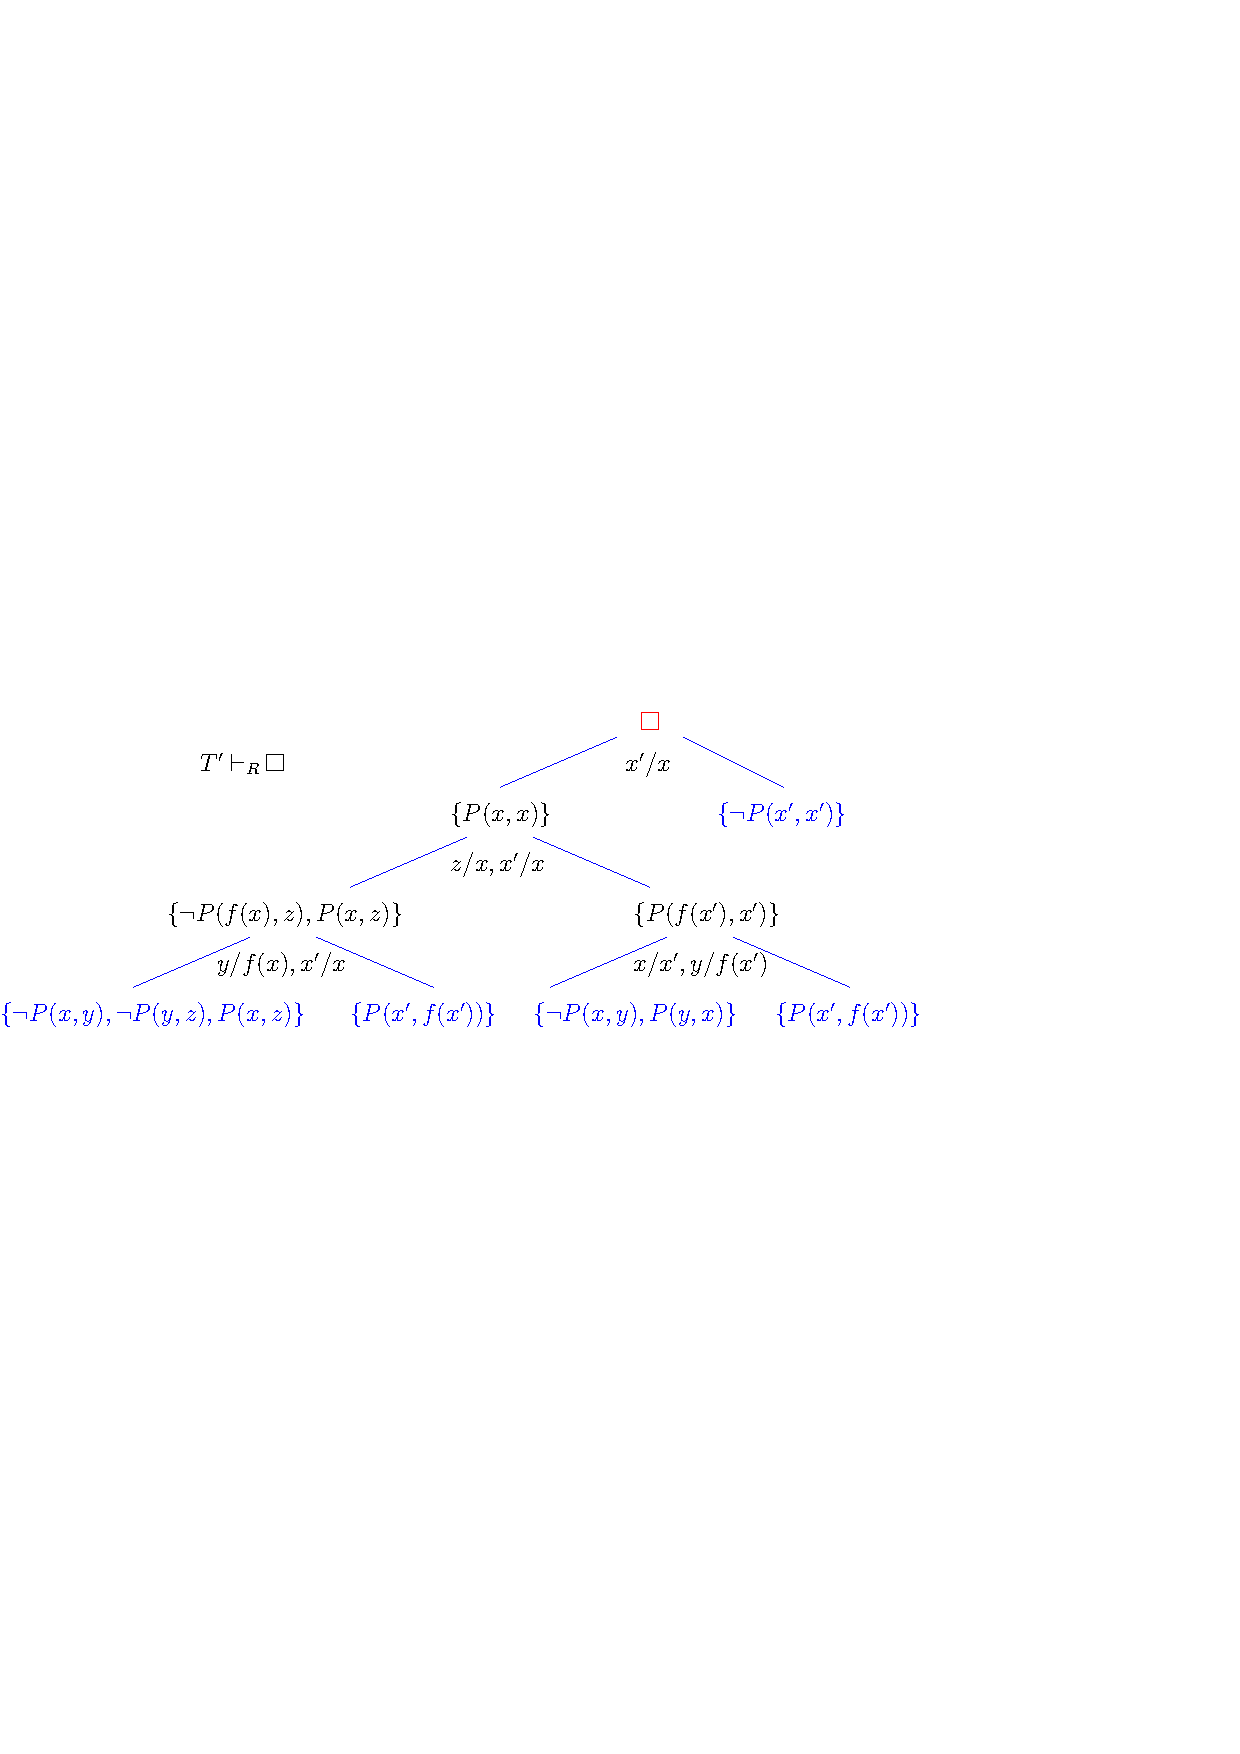
\includegraphics[scale=0.8]{files/rezolucePLpriklad}}
    
    
% :from slides


\section{Korektnost a úplnost}\label{section:predicate-resolution-soundness-completeness}
\todo

% from slides:

% :from slides

\subsection{Věta o korektnosti}\todo

% from slides:
{\it Nejprve ukážeme, že obecné rezoluční pravidlo je korektní.}
\medskip

{\bf \myblue{Tvrzení}}\ \ {Nechť $C$ je rezolventa klauzulí $C_1$, $C_2$. Pro každou $L$-strukturu $\mathcal{A}$,}
\vspace{-2mm}
$$\mathcal{A}\models C_1\ \ \text{a}\ \ \mathcal{A}\models C_2\quad \Rightarrow \quad \mathcal{A}\models C.$$

\vspace{-1mm}
{\it \myblue{Důkaz}}\ \ Nechť \mygreen{$C_1=C'_1\sqcup \{A_1,\dots,A_n\}$}, \mygreen{$C_2=C'_2\sqcup \{\neg B_1,\dots,\neg B_m\}$}, $\sigma$ je
\smallskip

nejobecnější unifikace pro \mygreen{$S=\{A_1,\dots,A_n,B_1,\dots,B_m\}$} a \mygreen{$C=C'_1\sigma \cup C'_2\sigma$}.
\smallskip

\begin{itemize}
\item Jelikož $C_1$, $C_2$ jsou otevřené, platí i $\mathcal{A}\models C_1\sigma$ a $\mathcal{A}\models C_2\sigma$.
\smallskip

\item Máme \mygreen{$C_1\sigma=C'_1\sigma \cup \{S\sigma$\}} a \mygreen{$C_2\sigma=C'_2\sigma \cup \{\neg(S\sigma)\}$}.
\smallskip

\item Ukážeme, že $\mathcal{A}\models C[e]$ pro každé $e$.
\smallskip
Je-li $\mathcal{A}\models S\sigma[e]$, pak $\mathcal{A}\models C'_2\sigma[e]$ a tedy $\mathcal{A}\models C[e]$.
\smallskip
Jinak $\mathcal{A}\not\models S\sigma[e]$, pak $\mathcal{A}\models C'_1\sigma[e]$ a tedy $\mathcal{A}\models C[e]$. $\qed$
\end{itemize}
\medskip

{\bf \myblue{Věta (korektnost)}}\ \ {\it Je-li formule $S$ rezolucí zamítnutelná, je $S$ nesplnitelná.}
\medskip

{\it \myblue{Důkaz}}\ \ Nechť $S \vdash_R \Box$. Kdyby $\mathcal{A}\models S$ pro nějakou strukturu $\mathcal{A}$, z korektnosti
\smallskip

rezolučního pravidla by platilo i $\mathcal{A} \models \Box$, což není možné. $\quad\mqed$
% :from slides

\subsection{Lifting lemma}\todo

% from slides:
\subsubsection*{Lifting lemma}
    {\it Rezoluční důkaz na úrovni VL lze ``zdvihnout'' na úroveň PL.}
    \medskip
    
    {\bf \myblue{Lemma}}\ \ {\it Nechť $C^*_1=C_1\tau_1$, $C^*_2=C_2\tau_2$ jsou \myblue{základní instance} klauzulí $C_1$, $C_2$
    \smallskip
    
    \myblue{neobsahující stejnou proměnnou} a $C^*$ je rezolventa $C^*_1$ a $C^*_2$. Pak existuje
    \smallskip
    
    rezolventa $C$ klauzulí $C_1$ a $C_2$ taková, že $C^*=C\tau_1\tau_2$ je základní instance $C$.}
    \medskip
    
    {\it \myblue{Důkaz}}\ \ Předpokládejme, že $C^*$ je rezolventa $C_1^*$, $C_2^*$ přes \myblue{literál}  $P(t_1,\dots,t_k)$.
    \vspace{0.5mm}
    
    \begin{itemize}
    \item Pak lze psát \mygreen{$C_1=C'_1 \sqcup \{A_1,\dots,A_n\}$} a \mygreen{$C_2=C'_2 \sqcup \{\neg B_1,\dots,\neg B_m\}$}, kde
    \smallskip
    
    \mygreen{$\{A_1,\dots,A_n\}\tau_1=\{P(t_1,\dots,t_k)\}$} a \mygreen{$\{\neg B_1,\dots,\neg B_m\}\tau_2=\{\neg P(t_1,\dots,t_k)\}$}.
    \smallskip
    
    \item Tedy $(\tau_1\tau_2)$ unifikuje $S=\{A_1,\dots,A_n,B_1,\dots,B_m\}$ a je-li $\sigma$ \myblue{mgu} pro $S$
    \smallskip
    
    z unifikačního algoritmu, pak \mygreen{$C=C'_1\sigma \cup C'_2\sigma$} je rezolventa $C_1$ a $C_2$.
    \smallskip
    
    \item Navíc $(\tau_1\tau_2)=\sigma(\tau_1\tau_2)$ z vlastnosti $(*)$ pro $\sigma$ a tedy
    \vspace{-2mm}
    \mygreen{\begin{align*}
    C\tau_1\tau_2&= (C'_1\sigma \cup C'_2\sigma)\tau_1\tau_2=C'_1\sigma\tau_1\tau_2 \cup C'_2\sigma\tau_1\tau_2=C'_1\tau_1 \cup C'_2\tau_2\\
    &=(C_1\setminus\{A_1,\dots,A_n\})\tau_1\cup (C_2\setminus\{\neg B_1,\dots,\neg B_m\})\tau_2\\
    &=(C_1^*\setminus\{P(t_1,\dots,t_k)\})\cup(C_2^*\setminus \{\neg P(t_1,\dots,t_k)\})=C^*. \qed
    \end{align*}}
    \end{itemize}
    
    
    \vspace{-8mm}
    
% :from slides

\subsection{Věta o úplnosti}\todo

% from slides:
\subsubsection*{Úplnost}
    {\bf \myblue{Důsledek}}\ \ {\it Nechť $S'$ je množina všech základních instancí klauzulí formule $S$.
    \smallskip
    
    Je-li $S'\vdash_R C'$ (na úrovni VL), kde $C'$ je základní klauzule, pak existuje
    \smallskip
    
    klauzule $C$ a základní substituce $\sigma$ t.ž. $C'=C\sigma$ a $S\vdash_R C$ (na úrovni PL).}
    \medskip
    
    {\it \myblue{Důkaz}}\ \ Indukcí dle délky rezolučního odvození pomocí lifting lemmatu. $\qed$
    \bigskip
    
    {\bf \myblue{Věta (úplnost)}}\ \ {\it Je-li formule $S$ nesplnitelná, je $S\vdash_R \square$.}
    \medskip
    
    {\it \myblue{Důkaz}}\ \ Je-li $S$ nesplnitelná, dle (důsledku) Herbrandovy věty je nesplnitelná i
    \smallskip
    
    množina $S'$ všech základních instancí klauzulí z $S$.
    \vspace{0.5mm}
    
    \begin{itemize}
    \item Dle úplnosti rezoluční metody ve VL je $S' \vdash_R \square$ (na úrovni VL).
    \smallskip
    
    \item Dle předchozího důsledku existuje klauzule $C$ a substituce $\sigma$ taková, že
    \smallskip
    
    $\square = C\sigma$ a $S\vdash_R C$ (na úrovni PL).
    \smallskip
    
    \item Jediná klauzule, jejíž instance je $\square$, je klauzule $C=\square$. \qed
    \end{itemize}
    
    
   
% :from slides


\section{LI-rezoluce}\label{section:predicate-LI-resolution}
\todo

% from slides:
\subsubsection*{Lineární rezoluce}
    {\it Stejně jako ve VL, rezoluční metodu lze značně omezit (bez ztráty úplnosti).}
    %\medskip
    
    \begin{itemize}
    \item \mdef{Lineární důkaz} klauzule $C$ z formule $S$ je konečná posloupnost dvojic
    \smallskip
    
     $(C_0,B_0),\dots,(C_n,B_n)$ t.ž. $C_0$ je \myblue{varianta} klauzule v $S$ a pro každé $i\le n$
    \smallskip
    
    \begin{enumerate}
    \item[{\normalsize $i)$}] {\normalsize $B_i$ je varianta klauzule v $S$ nebo $B_i=C_j$ pro nějaké $j<i$, a}
    \medskip
    
    \item[{\normalsize $ii)$}] {\normalsize $C_{i+1}$ je rezolventa $C_i$ a $B_i$, kde $C_{n+1}=C$.}
    \smallskip
    
    \end{enumerate}
    
    \item $C$ je \mdef{lineárně dokazatelná} z $S$, psáno $S \vdash_L C$, má-li lineární důkaz z $S$.
    \smallskip
    
    \item \mdef{Lineární zamítnutí} $S$ je lineární důkaz $\Box$ z $S$.
    \smallskip
    
    \item $S$ je \mdef{lineárně zamítnutelná}, pokud $S \vdash_L \Box$.
    \end{itemize}
    \medskip
    
    {\bf \myblue{Věta}}\ \ {\it $S$ je lineárně zamítnutelná, právě když $S$ je nesplnitelná.}
    \medskip
    
    {\it \myblue{Důkaz}}\ \ $(\Rightarrow)$ Každý lineární důkaz lze transformovat na rezoluční důkaz.
    \smallskip
    
    $(\Leftarrow)$ Plyne z úplnosti lineární rezoluce ve VL (nedokazováno), neboť lifting
    \smallskip
    
    lemma zachovává \myblue{linearitu} odvození. $\qed$
    %\medskip
    
    %{\it \myblue{Poznámka}\ \ Platí i \myblue{úplnost}, tj. je-li $S$ nesplnitelná, je $S$ lineárně zamítnutelná.}
    %Důkaz v dodatku.
    
    
    
    %%%%%%%%%%%%%%%%%%%%%%%%%%%%%%%%%%%%%%%%%%%%%%%%%%%%%%5
    
    \subsubsection*{LI-rezoluce}
    {\it Stejně jako ve VL, pro Hornovy formule můžeme lineární rezoluci dál omezit.}
    
    \begin{itemize}
    \item \mdef{LI-rezoluce} \emph{(``linear input'')} z formule $S$ je lineární rezoluce z $S$, ve které
    \vspace{0.5mm}
    
    je každá boční klauzule $B_i$ variantou klauzule ze (vstupní) formule $S$.
    \item Je-li klauzule $C$ dokazatelná LI-rezolucí z $S$, píšeme \mdef{$S\vdash_{LI} C$}.
    \smallskip
    
    \item \mdef{Hornova formule} je množina (i nekonečná) Hornových klauzulí.
    \item \mdef{Hornova klauzule} je klauzule obsahující nejvýše jeden pozitivní literál.
    \item \mdef{Fakt} je (Hornova) klauzule $\{p\}$, kde $p$ je pozitivní literál.
    \item \mdef{Pravidlo} je (Hornova) klauzule s právě jedním pozitivním a aspoň jedním
    \vspace{0.5mm}
    
    negativním literálem. Pravidla a fakta jsou \mdef{programové klauzule}.
    \item \mdef{Cíl} je neprázdná (Hornova) klauzule bez pozitivního literálu.
    \end{itemize}
    \smallskip
    
    {\bf \myblue{Věta}}\ \ {\it Je-li Hornova $T$ splnitelná a $T\cup \{G\}$ nesplnitelná pro cíl $G$, lze $\Box$
    \smallskip
    
    odvodit LI-rezolucí z $T\cup\{G\}$ začínající $G$.}
    \medskip
    
    {\it \myblue{Důkaz}}\ \ Plyne z Herbrandovy věty, stejné věty ve VL a lifting lemmatu. $\qed$
    
    
% :from slides

\subsection{(draft) Rezoluce v Prologu}\todo

% from slides:
\subsubsection*{Program v Prologu}
    \mdef{Program} (v Prologu) je Hornova formule obsahující pouze \myblue{programové}
    \smallskip
    
    \myblue{klauzule}, tj. \myblue{fakta} nebo \myblue{pravidla}.
    \bigskip
    
    \centerline{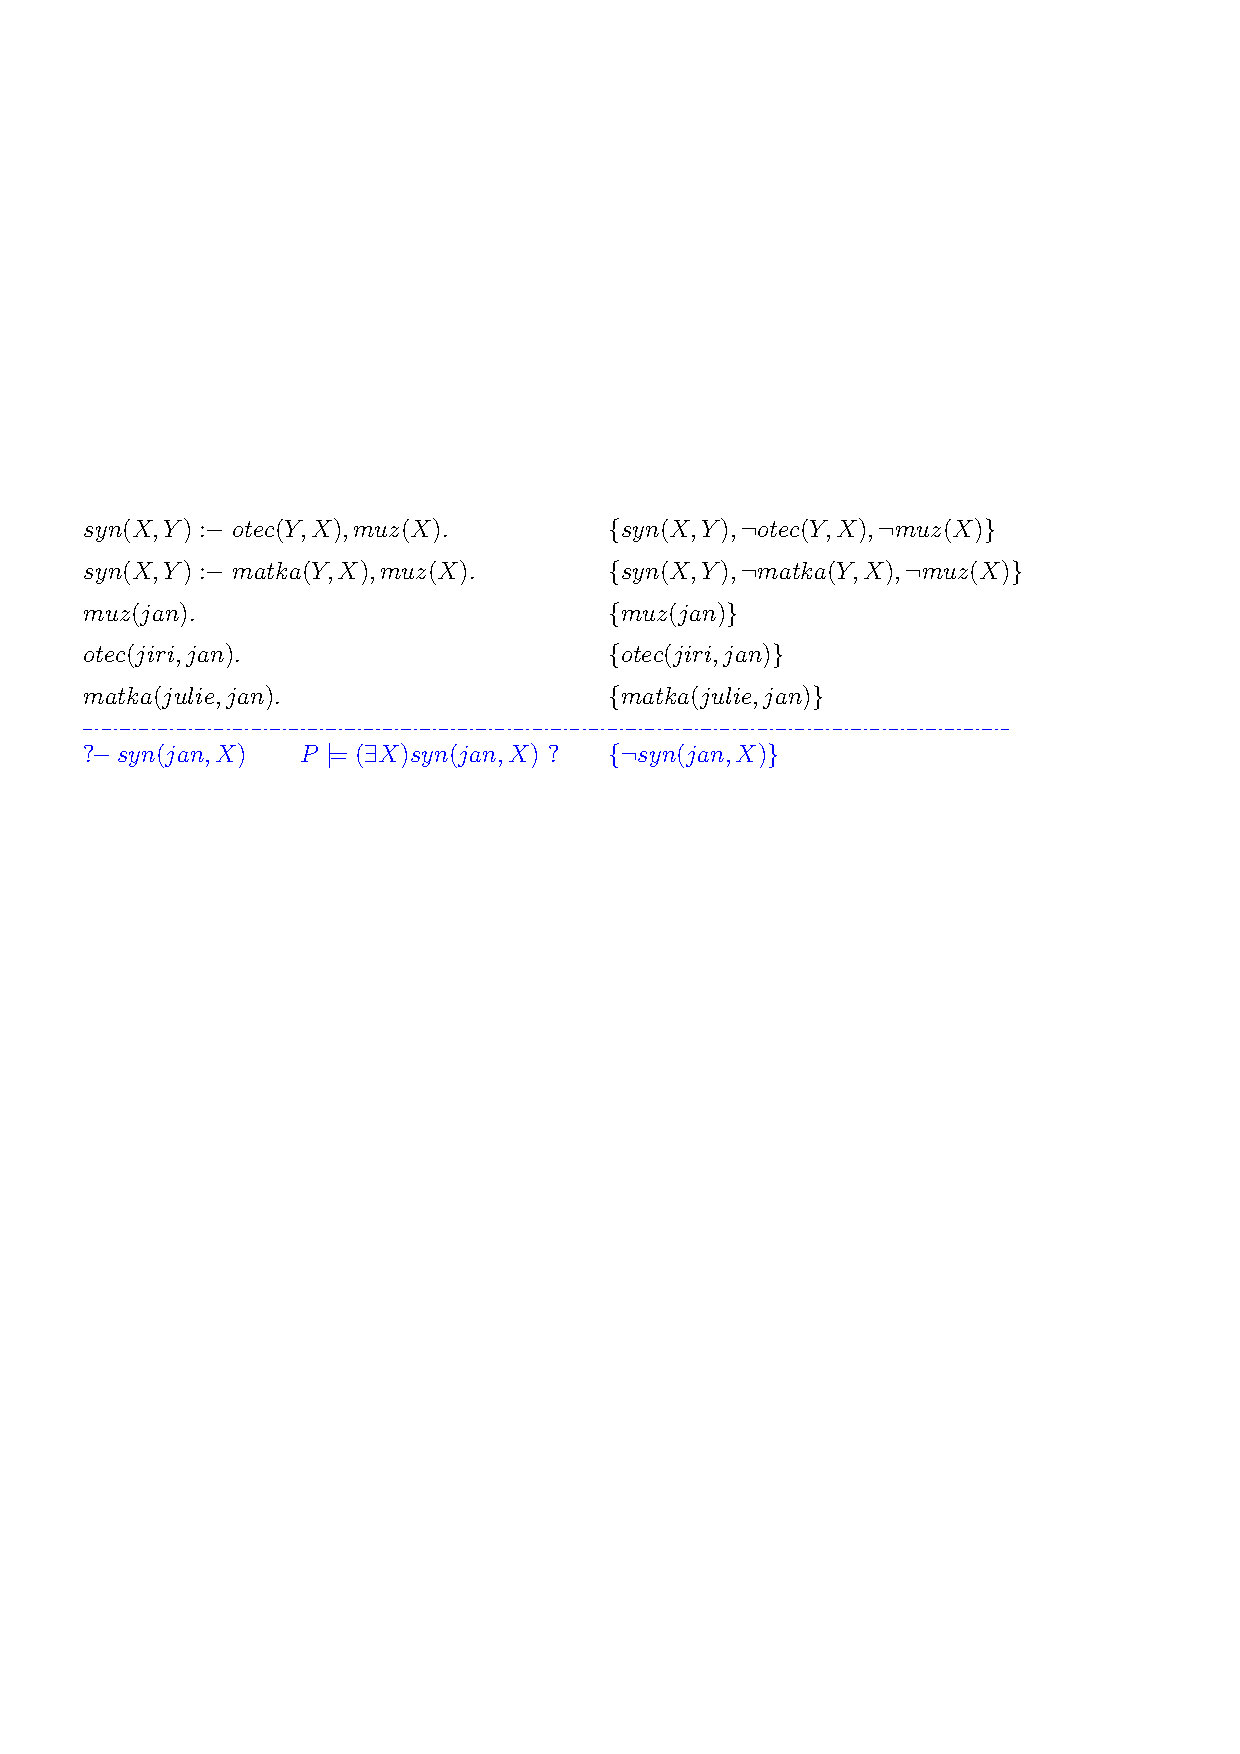
\includegraphics[scale=0.7]{files/rezolucePLprogram}}
    \bigskip
    
    {\it Zajímá nás, zda daný \myblue{existenční dotaz} vyplývá z daného programu.}%, navíc to chceme doložit \myblue{výstupní substitucí}.
    \medskip
    
    {\bf \myblue{Důsledek}}\ \ {\it Pro program $P$ a cíl $G=\{\neg A_1, \dots, \neg A_n\}$ v proměnných $X_1,\dots,X_m$
    
    \vspace{-0mm}
    \begin{enumerate}
    \item[$(1)$] $P \models (\exists X_1)\dots(\exists X_m)(A_1\mand \dots \mand A_n)$, právě když
    \smallskip
    
    \item[$(2)$] $\square$ lze odvodit LI-rezolucí z $P\cup\{G\}$ začínající (variantou) cíle $G$.
    \end{enumerate}}
    
    
    %%%%%%%%%%%%%%%%%%%%%%%%%%%%%%%%%%%%%%%%%%%%%%%%%%%%%%5
    
    \subsubsection*{LI-rezoluce nad programem}
    {\it Je-li odpověď na dotaz kladná, chceme navíc znát výstupní substituci.}
    \medskip
    
    \mdef{Výstupní substituce} $\sigma$ LI-rezoluce $\square$ z $P\cup\{G\}$ začínající $G=\{\neg A_1,\dots,\neg A_n\}$
    \smallskip
    
    je složení \myblue{mgu} v jednotlivých krocích (jen na proměnné v $G$). Platí,
    \vspace{-2mm}
    \mygreen{$$P \models (A_1 \mand \dots \mand A_n)\sigma.$$}
    
    \vspace{-2mm}
    
    \centerline{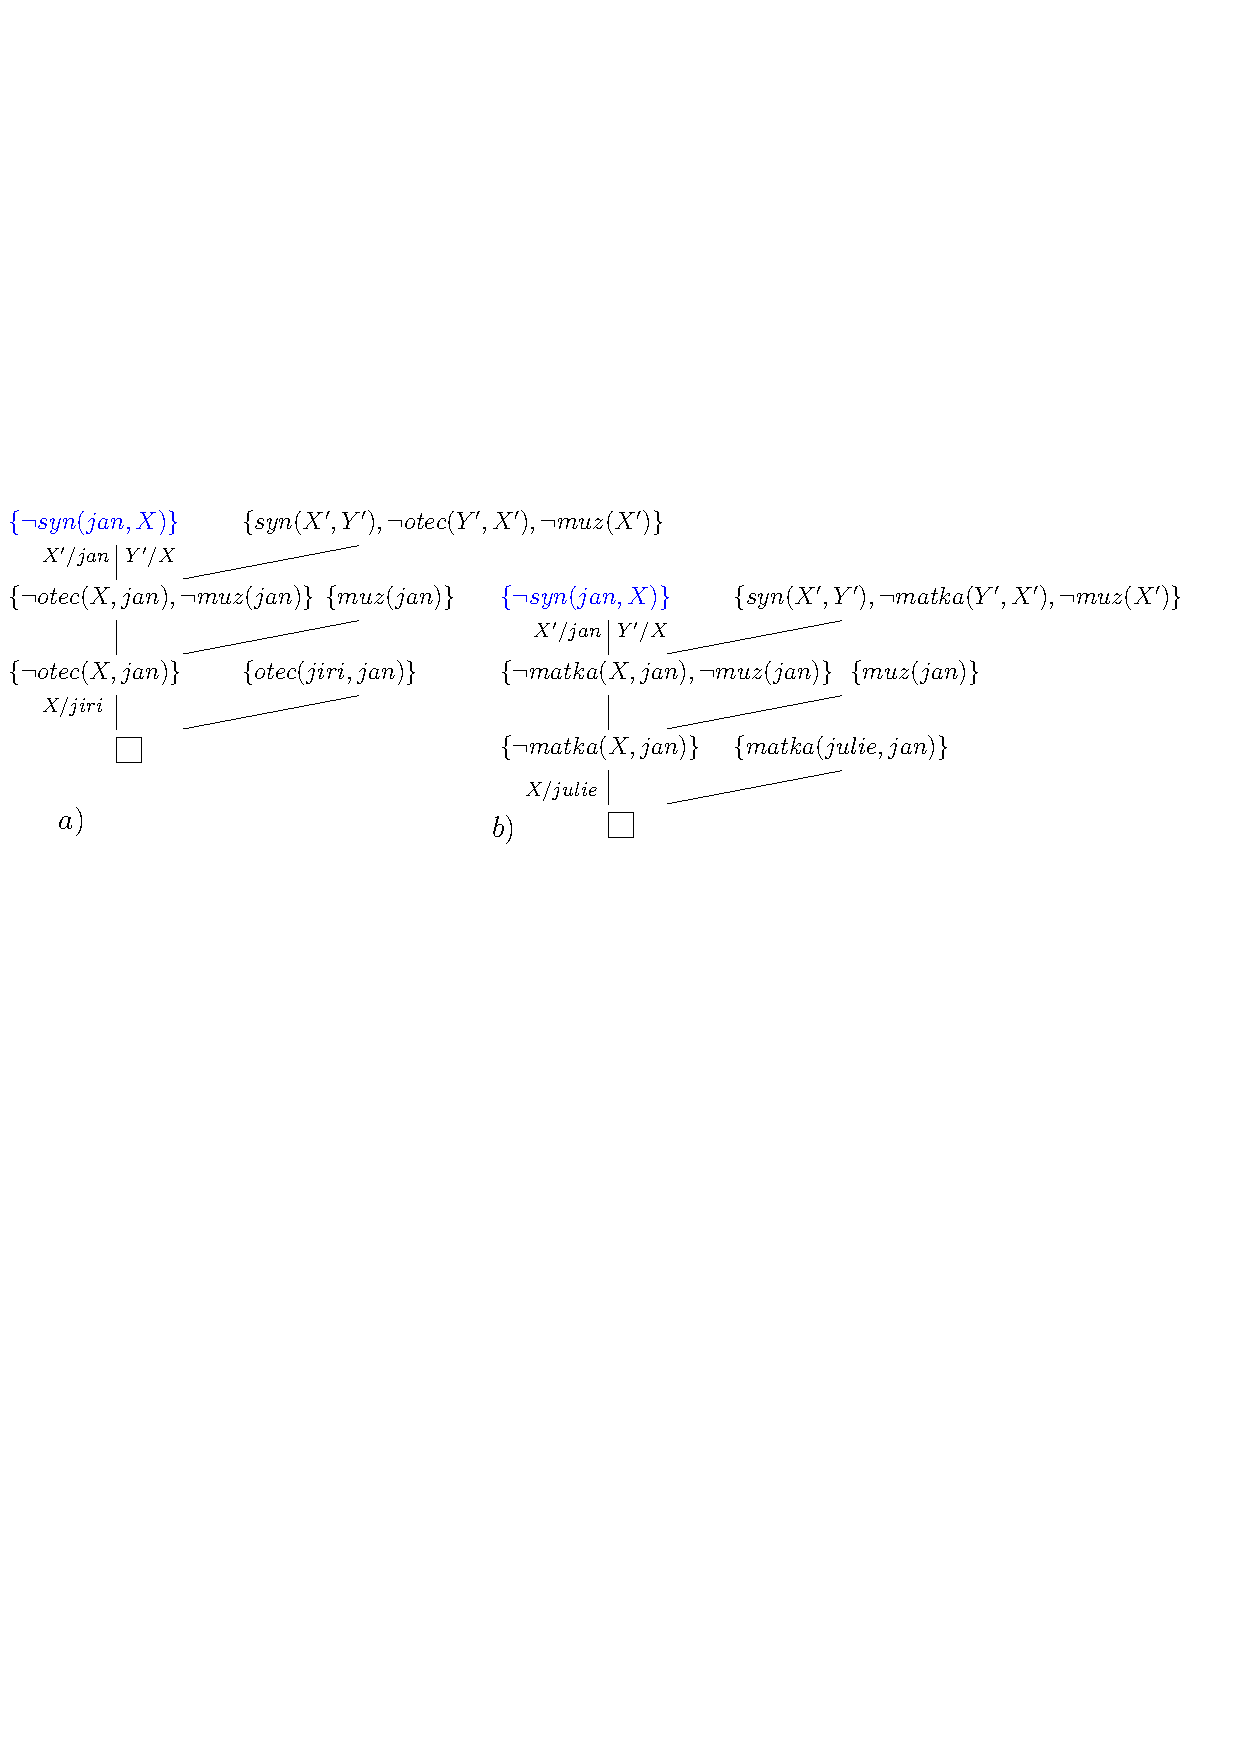
\includegraphics[scale=0.63]{files/rezolucePLprogramLI}}
    \bigskip
    
    Výstupní substituce $a)$ $X=jiri$,\ \ $b)$ $X=julie$.
    
    
% :from slides



